\chapter{La legge di Gauss}
\section{L'aspetto fisico}
Per calcolare il campo elettrico $\vec{E}$ di una distribuzione di carica si può \textbf{sommare} (integrare). La procedura è \textit{laboriosa}. Se esiste la simmetria, possiamo utilizzare un metodo più semplòice che sfrutta la relazione tra carica e campo, la \textbf{legge di Gauss}
\section{La superficie Gaussiana}
Scegliamo una superficie Gaussiana ({\it cioè una superficie chiusa}) intorno ad una carica.
Per la carica puntiforme, la {\bf sfera} è la superficie più simmetrica.
Le linee di campo intercettano la superficie.
\begin{tasks}
  \task Per una carica $Q$ il campo è $E=\frac{kQ}{r^2}$
  \task Per una carica 2Q, più linee intercettano la superficie
  \task la carica è $-\frac{Q}{2}$
\end{tasks}
Serve una grandezza che \textbf{quantifica} quanto una superificie è attraversata da un campo.
\section {Il flusso elettrico}
Un campo $\vec{E}$ attraversa un elemento di superficie $\Delta \vec{A}$ \texttt{vettore di area $\Delta \vec{A}$: \textbf{perpendicolare} alla superficie}.\\ Definizione del flusso elettrico $\Delta \vec{\upphi}$:
\begin{equation}
	\Delta \upphi =\vec{E}*\Delta\vec{A}=E\Delta A\cos\texttheta
\end{equation}
Per l'\textit{intera} superficie:
$\upphi = \sigma \vec{E}*\Delta \vec{A}=\int \vec{E}*d\vec{A}$ - Per una superficie chiusa, l'orientamento di $\Delta \vec{A}$ è uscente.
\begin{itemize}
\item $\vec{E}$ uscente contribuisce $\Delta \upphi >0$
\item $\vec{E}$ entrante contribuisce $\Delta \upphi <0$
\item $\vec{E} || \Delta \vec{A}$ da $\Delta \upphi =0$
\end{itemize}
Il flusso netto di una superficie chiusa è
\begin{equation}
	\upphi=\oint \vec{E}*d\vec{A}
\end{equation}
\section{Cilindro in campo uniforme}
Superficie guessiana a forma di \textbf{cilindro} di raggio \textit{R}. Campo elettrico $\vec{E}$
\textbf{uniforme}, parallelo all'asse. Quanto vale il fluso netto?
\begin{equation}
  \upphi=\oint \vec{E}*d\vec{A}=\int_a \vec{E}*d\vec{A}+\int_b\vec{E}*d\vec{A}+\int_c \vec{E}*
  d\vec{A}
\end{equation}
\begin{itemize}
\item $\int_a \vec{E}*d\vec{A}=-\pi R^2E$
\item $\int_b \vec{E}*d\vec{A}=0$
\item $\int_c\vec{E}*d\vec{A}=\pi R^2E$
\item $\upphi =0$  
\end{itemize}
\section{La legge di Gauss}
Relazione tra il flusso $\upphi$ attraverso una superficie chiusa e la carica netta $q_{int}$ racchiusa all'interno della superficie:
\begin{equation}
	\xi_0\upphi=q_{int} \text{ o } \xi_0\oint \vec{E}*d\vec{A}=q_{int}
\end{equation}
\begin{itemize}
\item \textit{se $q_{int}$ è positiva, il flusso netto è uscente}
\item \textit{se $q_{int}$ è negativo, il flusso netto è entrante}
\end{itemize}
Una carica esterna alla superficie può cambiare $\vec{E}$ localmente, ma non influisce sul flusso totale.
\begin{figure}[!h]
 	\centering
	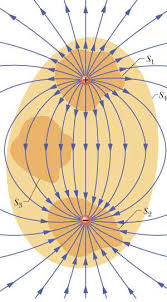
\includegraphics[height=5cm]{img/cariche opposte.jpg}
    	\caption{Due cariche di intensità uguale, ma di segno opposto}
\end{figure}
\begin{itemize}
\item $S_1$: $\vec{E}$ uscente in tutti i punti. $\Phi$ positivo, $q_{int}$ negativa
\item $S_2$: $\vec{E}$ entrante in tutti i punti. $\Phi$ negativa, $q_{int}$ negativa
\item $S_3$ Non racchiude nessuna carica. Ogni linea di campo che entra, esce, quindi $\Phi = 0$
  \item $S_4$ $q_{int}$ = $Q-Q=0$, quindi $\Phi = 0$
\end{itemize}

\section{La legge di Gauss e di Coulomb}
Racchiudiamo una \textbf{carica puntiforme} in una superficie sferica di raggio $r$.
Per simmetria, il campo elettronico ha il medesimo modulo $E$ su \textbf{tutti i punti della sfera}.\\
Applichiamo Gauss:
\begin{eqnarray*}
  \xi_0\oint \vec{E}*d\vec{A}=q_{int}\\
  \xi_0 E(4\pi r^2) = q\\
  E=\frac{q}{4\pi\xi_0r^2}
\end{eqnarray*}
Cioè, la legge di coulomb!
\subsection{Problema svolto}
Guscio sferica di raggio $R=10cm$ - dotato di carica uniforme $Q=-16e$ - Al centro carca puntiforme $q=5e$. Calcolare il campo $\vec{E}$
\begin{itemize}
\item nel punto $P_1$ a $r_1=6cm$
\item nel punto $P_2$ a $r_2=12cm$
\end{itemize}
\begin{eqnarray*}
  \xi_0 E_1(4\pi r_1^2)=q\to E=\frac{q}{4\pi \xi_0 r^2_1}=\frac{4e}{4\pi \xi_0 (0,06m)^2}=2,0*10^{-6}\frac{N}{C} \text{ verso l'esterno}\\
  \xi_0 E_2 (4\pi r^2_2)=q+Q\to \frac{q+Q}{4\pi \xi_0 r^2_2}=\frac{4e}{4\pi \xi_0 (0,12m)^2}=1,1 *10^{-6}\frac{N}{C} \text{ verso l'interno}
\end{eqnarray*}
\section{Un conduttore carico isolato}
Il campo elettrico all'\textit{interno} di un conduttore in equilibrio elettrostatico è \textit{nullo}
\begin{center}
	se no, si spostano le cariche
\end{center}
Scegliamo una superficie gaussiana appena sotto la superficie. $E=0\to \phi=0\to q_{int}=0$\\
L'eccesso di carica su un conduttore isolato si dispone totalmente sulla
\textbf{superficie esterna}. Anche una superficie gaussiana che racchiude \textbf{una cavita} ha
$E=0 \to \phi=0\to q_{int}=0$. La superficie di una cavità interna di un conduttore \textbf{non ha carica} in eccesso.\\
In generale, la carica \textit{non} si distribuisce uniformemente sulla superficie di un conduttore. Però c'è una relazione diretta tra il \textbf{campo} \textit{E} e la \textbf{densità di carica} $\sigma$. Considera un ciindro che racchiude un elemento di superficie - Il campo $E$ è
\textbf {perpendicolare} alla superficie
\begin{center}
	{\it se no si sposta la carica}
\end{center}
applicando Gauss: $\xi_0 \oint \vec{E}*d\vec{A}=q_{int}\to \xi_0EA=\sigma A \to E=\frac{\sigma}{\xi_0}$
\subsection{Problema svolto}
Una carica puntiforme di $Q=-5\mu C$ è posta all'interno di un guscio sferico metallico di raggio interno $R$, spostato di una distanza $\frac{R}{2}$ dal centro.
\begin{itemize}
\item Qual'è la carica indotta?
\item Qual'è l'andamento del campo interno ed esterno?
\end{itemize}
$Q$ induce un carica positiva $+5\mu C$ di all'interno, distribuita in modo \textbf{non-uniforme}.
Il campo all'interno è asimmetrico. La parete interna ha una carica di $-5\mu C$ distribuita in modo \textbf{uniforme}. Il campo esterno è simmetrico, come il campo di una carica puntiforme.
\section{Gauss per simmetria cilidrica}
Una bacchetta di plastica, di lunghezza infinita, densità di carica pari a $\lambda C/m$, Com'è il campo $\vec{E}$ a distanza $r$? Fruttare l'integrale è davvero faticoso\dots Applichiamo Gausss per la \textbf{superficie cilintrica} di altezza $h$. Per simmetria, $\vec{E}$ ha direzione \textbf{radiale}.
\begin{equation}
\xi_9\oint \vec{E}*d\vec{A}=q_{int}\to \xi_0 E2\pi hr=\lambda h\to E=\frac{\lambda}{2\pi r\xi_0}
\end{equation}
vake se la distanza dell'estremità è molto minore di $r$.
\section{Gauss per simmetria piana}
Una lamina isolante sottile, con una densità di carica superficiale $\sigma \frac{C}{m^2}$.
\paragraph{Superficie gaussiana:} cilindro di base $A$. Per simmetria, $\vec{E}$ perpendicolare alla lamina.\\ Applichiamo Guass: $\xi \oint \vec{E}*d\vec{A}=q_{int} \to \xi_0E2A=\sigma A\to E=\frac{\sigma}{2\xi_0}$\\
Concorda con il risultato trovato per il disco $E=\frac{\sigma}{2\xi_0}\left(1-\frac{z}{\sqrt{(R^2+z^2)}}\right)$\\
Per una piastra conduttrice la carica si distribuisce sulla superficie. Senza campo esterno, la carica è uguale da ambi lati, $\sigma_1=\sigma/2$. Identico, ma con verso di $E$ opposto, per carica negativa. Messe una a cando all'altra, le cariche sono attratte verso l'intrno. Il campo in mezzo diventa $E=\frac{2\sigma_1}{\xi_0}=\frac{\sigma}{\xi_0}$
\section{Gauss per simmetria sferica}
Con Gauss dimostriamo i 2 teoremi dei gusci. Guscio sferico di carica totale $q$ e raggio $R$.
\begin{enumerate}
\item \textit{Una superficie unifomemente carica attrae o respinge una carica esterna come se tutta la carica fosse concentrata nel suo centro.} Applicare Gauss alla superficie $S_2: E=\frac{q}{4\pi \xi_0 r^2}$ per $(r>R)$
  \item \textit{Una carica posta all'interno di una superficie chiusa uniformemente carica non ne sente la forza.} Applicare Gauss alla superficie $S_2: E=q_{int}=0$ per $(r<R)$
\end{enumerate}
Ogni distribuzione con simmetira sfrefica è una sovrapposizione di strati concentrici. Densità di carica $p$ varia soltanto con $r$
\begin{equation}
  E=\frac{q^\prime}{4\pi\xi_0r^2}
\end{equation}
Per $p$ uniforme e $r<R$
\begin{equation}
  	\frac{q^\prime}{\frac{4}{3}\pi r^3}=\frac{q}{\frac{4}{3}\pi R^3}\to q^\prime=q\frac{r^3}{R^3}
\end{equation}
per ci $E=\frac{qr}{4\pi \xi_0 R^3}$
